\documentclass[12pt]{article}
\usepackage{amsmath}
\usepackage{listings}
\usepackage{enumerate}
\usepackage{color}
\usepackage{graphicx}
\usepackage[margin=0.5in]{geometry}
\title{Project 3}

\author{Dan Kolbman}
\date{December 5, 2014}

\definecolor{mygreen}{rgb}{0,0.6,0}
\definecolor{mygray}{rgb}{0.95,0.95,0.95}
\definecolor{mymauve}{rgb}{0.58,0,0.82}
%\definecolor{mygray}{RGB}{22, 22, 22}}

\lstset{ %
  language=Python,
  backgroundcolor=\color{mygray},   % choose the background color
  basicstyle=\footnotesize,        % size of fonts used for the code
  breaklines=true,                 % automatic line breaking only at whitespace
  captionpos=b,                    % sets the caption-position to bottom
  commentstyle=\color{mygreen},    % comment style
  %escapeinside={\%*}{*)},          % if you want to add LaTeX within your code
  keywordstyle=\color{blue},       % keyword style
  stringstyle=\color{mymauve},     % string literal style
  frame=L,
  xleftmargin=\parindent,
  showstringspaces=false
}
\begin{document}
  
  \maketitle

  \section{Lane-Emden Equation}
  \begin{figure}[h!]
    \centering
    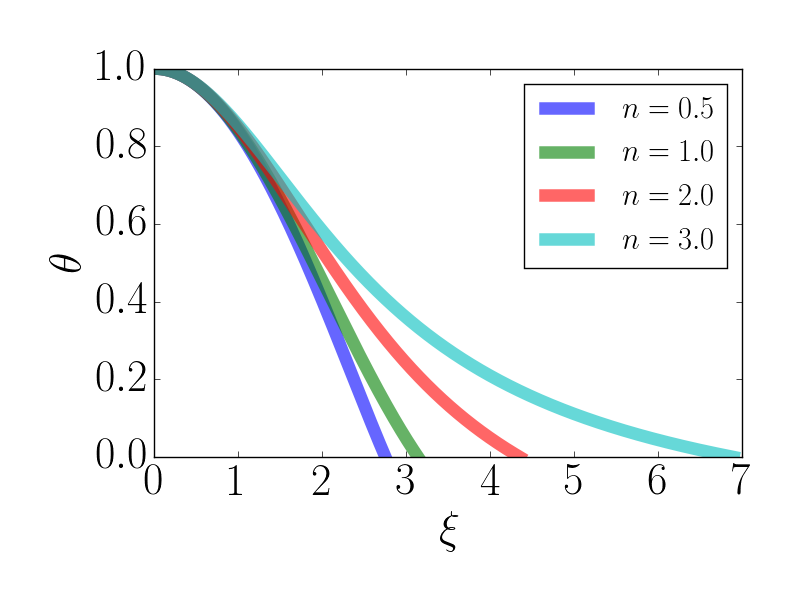
\includegraphics[width=1.0\textwidth]{lane-emden.png}
    \caption{Lane-Emden for $n=0.5,1,2,3$}
  \end{figure}
  \clearpage
  \section{Dimensionless Quantities}
  \begin{table}[h!]
    \begin{center}
      \begin{tabular}{ | c | c | c | c | c | c | }
        \hline
        $n$ & $\hat{M}$  & $\Xi$  & $-(\frac{d\theta}{d\xi})_{\xi=\Xi}$ & $ \hat{\Omega} $ & $\hat{I}$ \\
        \hline
        0.5 & 47.5911 & 2.7528 & 0.4999 & 1.7268 & 0.1764 \\
        \hline
        1   & 39.4651 & 3.1419 & 0.3182 & 2.0003 & 0.2612 \\
        \hline
        2   & 30.2913 & 4.3537 & 0.1271 & 2.8059 & 0.5792 \\
        \hline
        3   & 25.3594 & 6.8999 & 0.0423 & 4.4188 & 1.5481 \\
        \hline
      \end{tabular}
      \caption{Dimensionless Quantities for different models}
    \end{center}
  \end{table}

  \begin{figure}[h!]
    \centering
    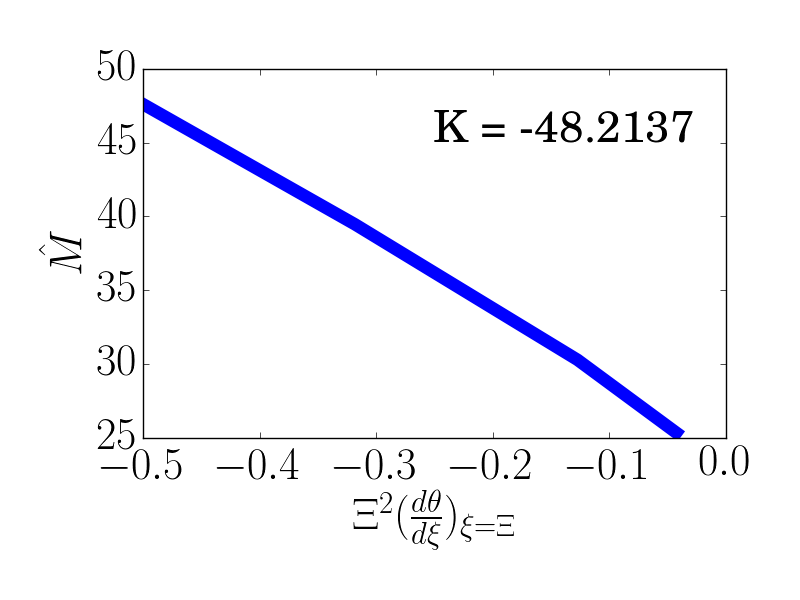
\includegraphics[width=0.6\textwidth]{K.png}
    \caption{Constant K from the slope}
  \end{figure}
 
  \clearpage 
  \section{Central Pressure of Sun}

  Using cgs units:
  \begin{align}
    G       &= 6.674e-8 \frac{cm^3}{g s} \nonumber  \\
    R_\sun  &= 695.8e8  cm \nonumber \\
    M_\sun  &= 1.989e33 g  \nonumber \\
    \hat{M} &= 25.3594   \nonumber \\
    \alpha  &= 1.0084e11 \nonumber \\
    \rho_c  &= \frac{M}{\alpha^3\hat{M}} \nonumber \\
            &= 0.07648    \nonumber \\
    \kappa  &= \alpha ^2\frac{4\pi G}{n+1}\frac{1}{\rho_c^{(1-n)/n}} \nonumber \\
            &= 1.9200e14  \nonumber \\
    P_c     &= 1.2473e17  \nonumber
  \end{align}

  $P_c$ from the $n=3$ model is more than half the expected value.

  \section{White Dwarfs}
  
  Defining $G(\theta)$ as:
  \begin{equation}
    G(\theta) \equiv \frac{\theta^{-1/3}(4\theta^{2/3}+5)}{3(\theta^{2/3}+1)^{3/2}} \nonumber
  \end{equation}
  We can solve:
  \begin{equation}
    \theta^{\prime\prime}G(\theta) + \frac{2}{s}G^\prime(\theta)(\theta^\prime)^2+\theta=0 \nonumber
  \end{equation}

  \begin{figure}
    \centering
    \begin{subfigure}
      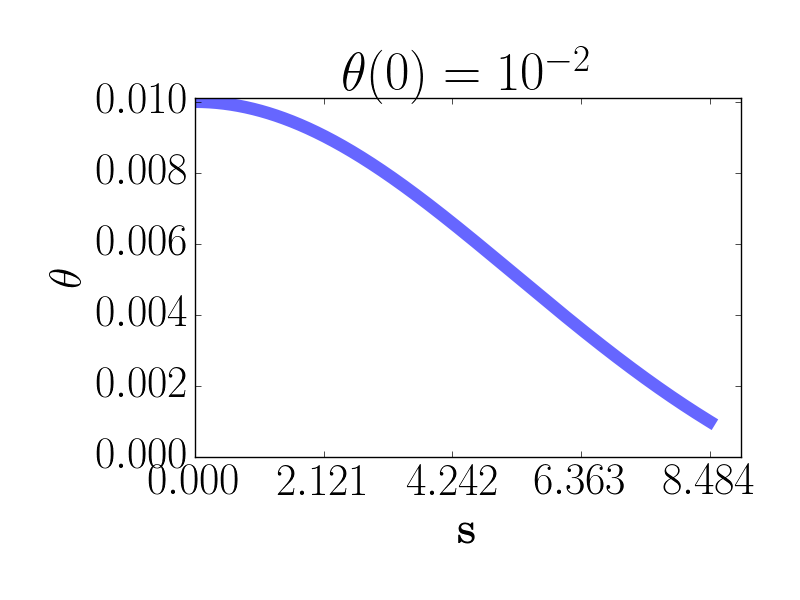
\includegraphics[width=0.3\textwidth]{white_dwarf-1.png}
    \end{subfigure}
    \begin{subfigure}
      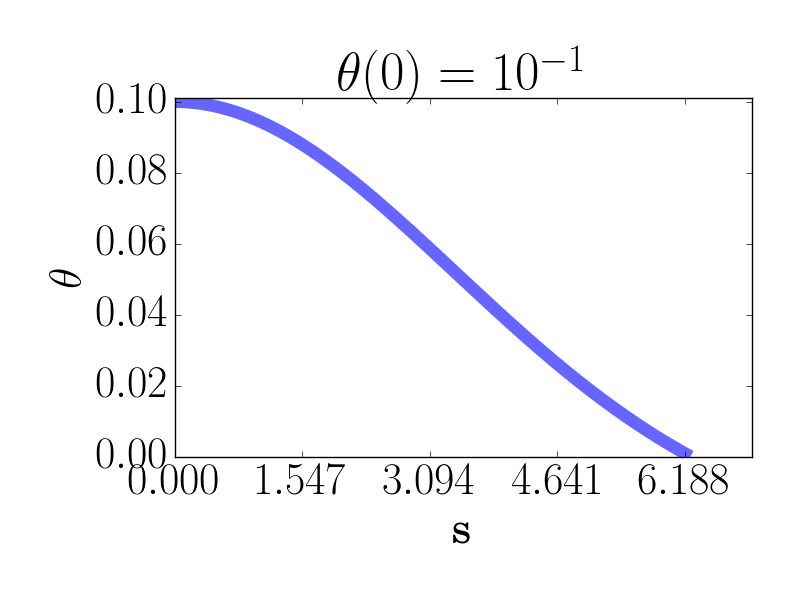
\includegraphics[width=0.3\textwidth]{white_dwarf-2.png}
    \end{subfigure}
    \begin{subfigure}
      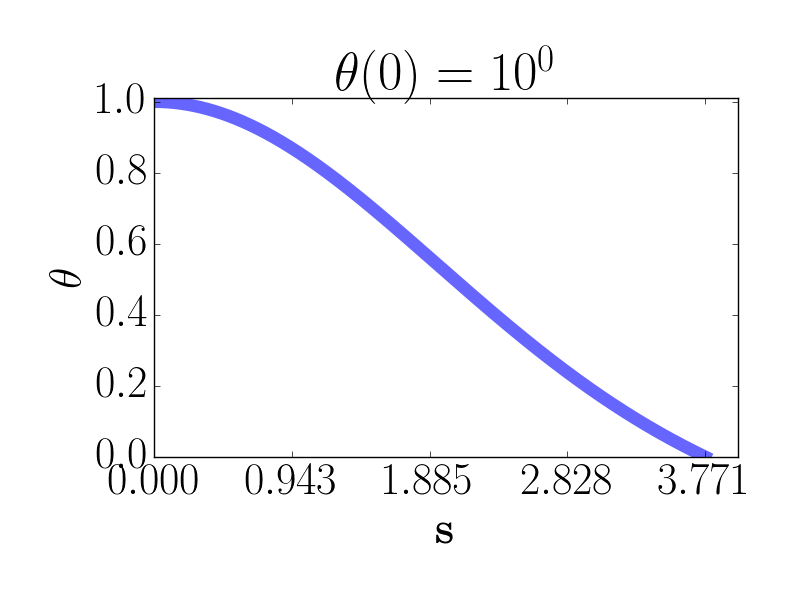
\includegraphics[width=0.3\textwidth]{white_dwarf-3.png}
    \end{subfigure}
    \begin{subfigure}
      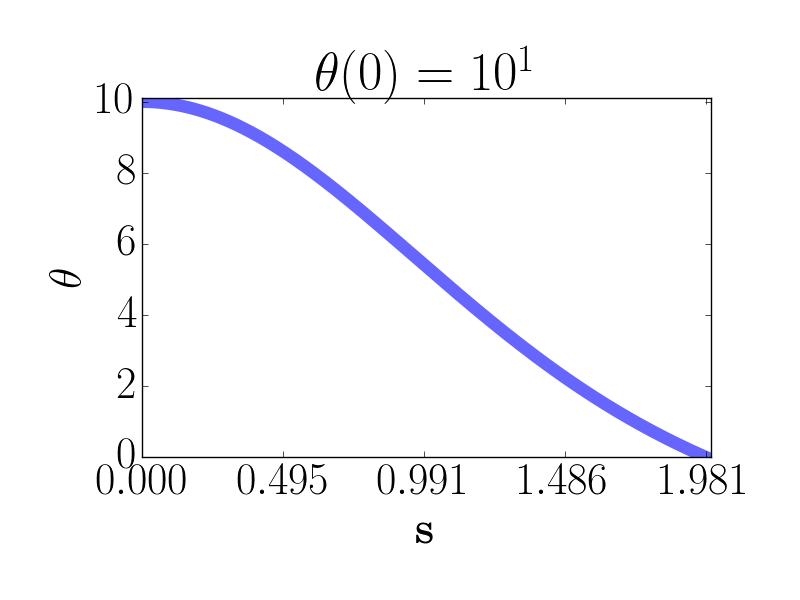
\includegraphics[width=0.3\textwidth]{white_dwarf-4.png}
    \end{subfigure}
    \begin{subfigure}
      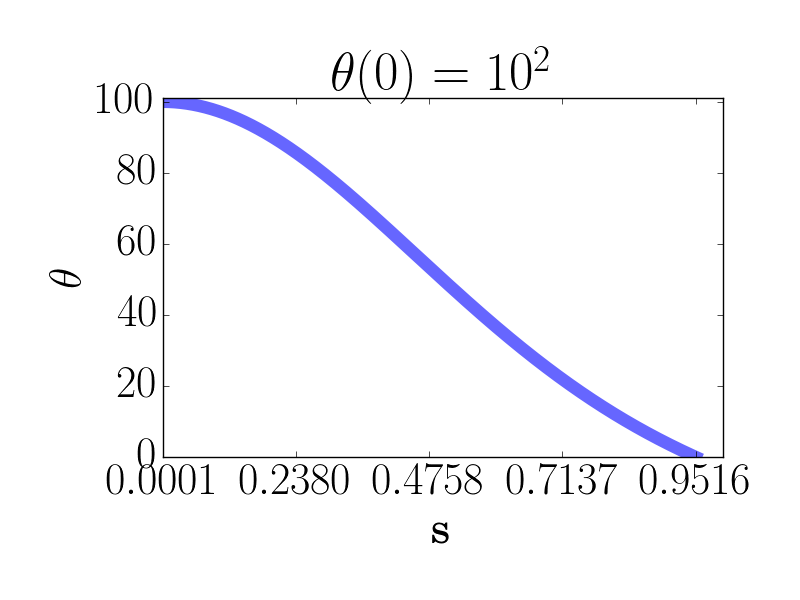
\includegraphics[width=0.3\textwidth]{white_dwarf-5.png}
    \end{subfigure}
    \begin{subfigure}
      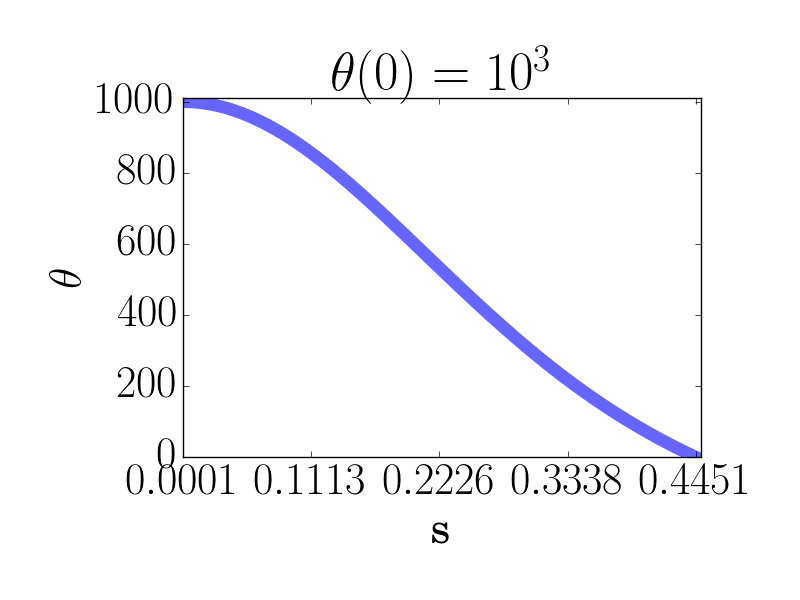
\includegraphics[width=0.3\textwidth]{white_dwarf-6.png}
    \end{subfigure}
    \begin{subfigure}
      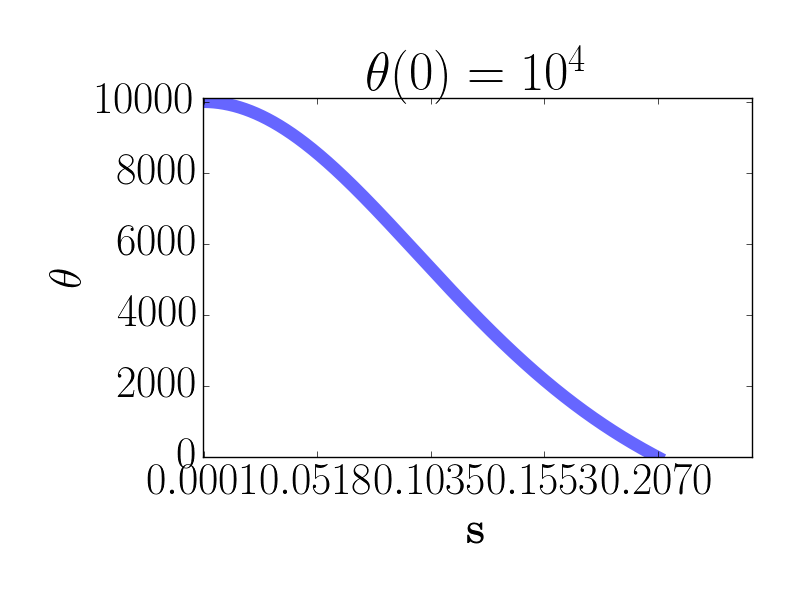
\includegraphics[width=0.3\textwidth]{white_dwarf-7.png}
    \end{subfigure}
    \begin{subfigure}
      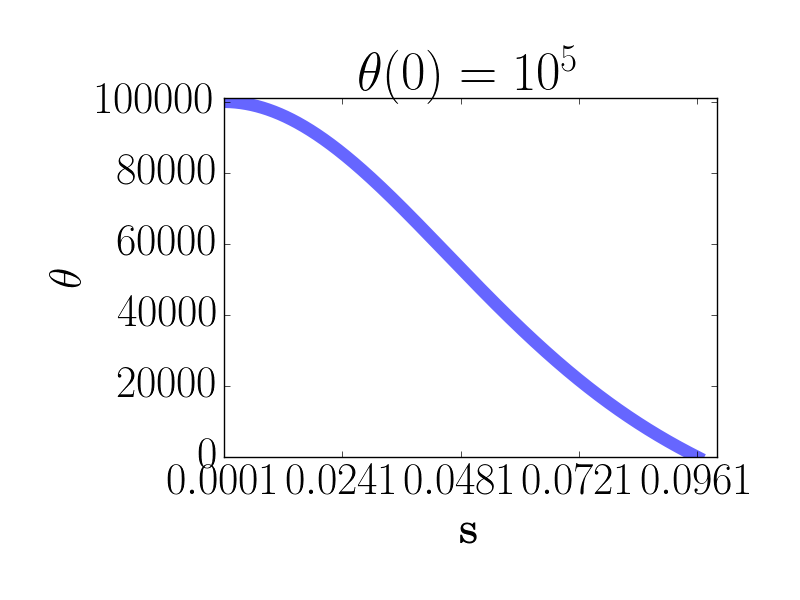
\includegraphics[width=0.3\textwidth]{white_dwarf-8.png}
    \end{subfigure}
  \end{figure}
  
  \begin{figure}[h!]
    \centering
    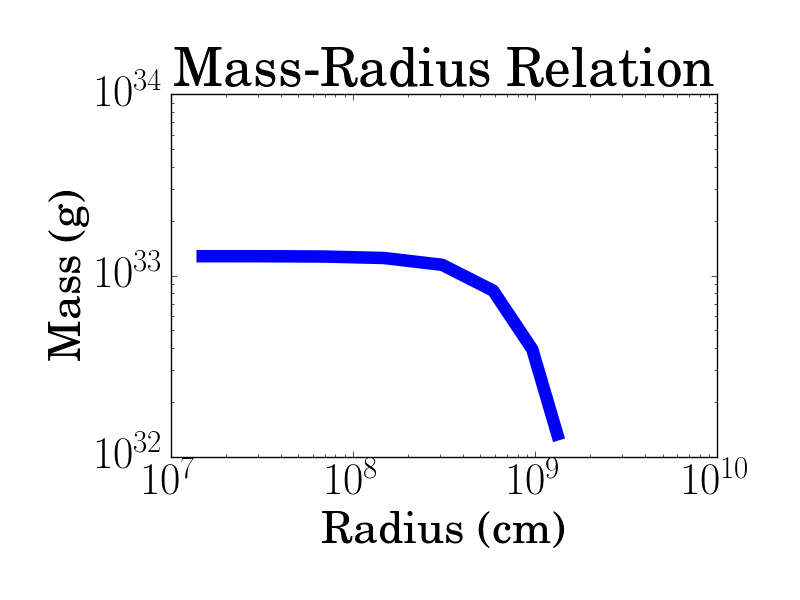
\includegraphics[width=0.6\textwidth]{massradius.png}
  \end{figure}

  
\end{document}
